\section{Repositories} \label{sc:RepositoryPatern}
To ensure the system is not hard-coded to utilize a specific database system, the repository pattern \citep{RepositoryPattern}. The repository pattern is used to create a uniform interface and connect the database to the rest of the system. As long as any database access component implements the repository-interfaces, it can connect to any version of any database system, if the implementation of the repository pattern is changed.
\par
The repository pattern encapsulates the functionality of creating, updating, reading, and deleting data within the database.
\par
This implementation has been a focus area, to make it easier for Aalborg Zoo to move to another database structure or platform at a later date, if necessary.
\par
The system specific structure of the implementation can be seen in \autoref{fig:RepositoryDiagram}.

\begin{figure}[H]
    \centering
    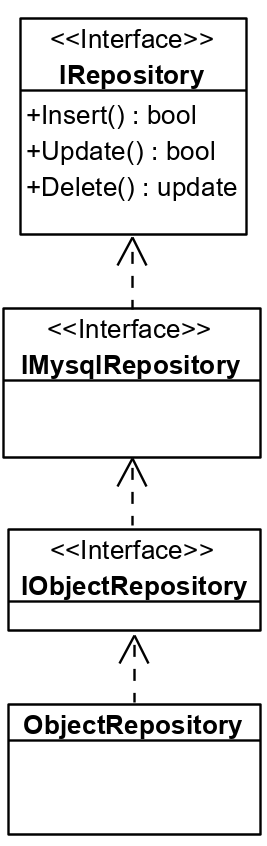
\includegraphics[width=0.2\textwidth]{figures/Implementation/GenericRepositoryStructure.PNG}
    \caption{Repository diagram}
    \label{fig:RepositoryDiagram}
\end{figure}

Any database access implemented by the system needs to implement the different interfaces. As seen in \autoref{fig:RepositoryDiagram} all of the database related repositories depend on \textit{IRepository}. This is done to ensure that the database interfaces implement \textbf{\textit{Insert()}}, \textbf{\textit{Update()}} and \textbf{\textit{Delete()}} as functions. By implementing the \autoref{code:IRepository} interface the database access implementation, satisfies the general needs for database access implementations.

\begin{listing}[H]
\begin{minted}[frame=lines, framesep=3mm, baselinestretch=1, linenos, bgcolor=LightGray, escapeinside='', breaklines]{csharp}
public interface IRepository<T>
{
    bool Insert(T entity, out ulong id);
    bool Update(T entity);
    bool Delete(T entity);

    T GetById(ulong id);
}

\end{minted}
\captionof{listing}{IRepository example.}
\label{code:IRepository}
\end{listing}
\par
Depending on which repository is used (\textit{Asset}, \textit{Log}, \textit{Tag}, etc.) different functionalities need to be implemented. 
\par
The interfaces on the third layer of \autoref{fig:RepositoryDiagram} (\textit{IObjectRepository}) define the functionalities specific to the objects, which the individual repository classes should implement. These classes handle the communication with the database, as well as constructing the SQL scripts to fit the specific model. As some of the models have unique ways of being searched, added or edited in the database, individual interfaces were needed for these, to make sure the objects were saved and loaded correctly.
\par
At the bottom of \autoref{fig:RepositoryDiagram}, the concrete object repository is defined. This class contains all the information and functions related to a specific model, defined in the chain of interfaces.
\par
If a new database structure were to be added at a later date, it would have to define a dependency to the last of the \textit{ObjectRepository}, and will thereby be forced to implement the required functions, to make the database connection useful.
